\documentclass[11pt]{article}
\usepackage[margin=1in]{geometry}
\usepackage{graphicx}
\usepackage{booktabs}
\usepackage{amsmath}
\usepackage{amssymb}
\usepackage{hyperref}
\usepackage{xcolor}
\usepackage[numbers,square]{natbib}

\title{ENACT: End-to-End Analysis of Visium High Definition Spatial Transcriptomics Data via Cell Segmentation and Bin-to-Cell Assignment}
\author{}
\date{}

\begin{document}
\maketitle

\begin{abstract}
Sequencing-based spatial transcriptomics has historically lacked the resolution required to resolve individual cells, and the recently released Visium High Definition (HD) platform only partially closes that gap: its $2\,\mu\mathrm{m}\times 2\,\mu\mathrm{m}$ bins are smaller than a cell, but the $8\,\mu\mathrm{m}\times 8\,\mu\mathrm{m}$ aggregated spots offered to users rarely align with a single cell. Existing methods that combine imaging and sequencing, such as Bin2cell with Stardist-based outlines, recover per-cell transcript counts when cells are isolated but degrade sharply when cells are tightly packed and a single bin overlaps multiple cells. We developed ENACT, a tissue-agnostic end-to-end pipeline that couples deep-learning cell segmentation (Stardist) with four alternative bin-to-cell assignment strategies---a Naive method and three weight-based variants---and three downstream cell-type annotation engines (Sargent, CellAssign, CellTypist). ENACT emits AnnData objects directly consumable by Squidpy for neighbourhood enrichment, Moran's I and co-occurrence analyses. On a Xenium-derived synthetic dataset with whole-cell boundaries, approximately 25\% of bins overlap more than one cell: in this regime Weighted-by-Area achieves the highest F1 score whereas the Naive method trades recall for precision. On a seqFISH+-derived synthetic dataset only about 5\% of bins overlap more than one cell and all four assignment methods reach precision close to 1 and recall close to 0.99. Evaluated against 20{,}991 pathologist-annotated cells, the Sargent and Weighted-by-Area combination yields accuracy 0.708 and weighted F1 0.758, and the predicted cell types agree with anatomical landmarks in human colorectal cancer and mouse small intestine tissues. ENACT turns Visium HD bin matrices into curated, spatially-resolved cell-type maps at scale.
\end{abstract}

\section{Introduction}

Spatial transcriptomics is an emerging class of technologies that couples gene expression measurement with the spatial organisation of tissue, allowing investigators to relate transcriptional state to histological context. These technologies are commonly grouped into two families. Sequencing-based methods, such as the original Spatial Transcriptomics platform~\cite{stahl2016spatialtranscriptomics} and its commercial successors including Visium, deposit barcoded spots on a slide and read transcripts with short-read sequencing. Imaging-based methods, such as MERFISH~\cite{chen2015merfish,moffitt2018merfish}, seqFISH+~\cite{eng2019transcriptome}, and the commercial Xenium platform~\cite{janesick2023xenium,rao2021xenium}, localise a targeted panel of transcripts through successive rounds of fluorescent hybridisation. Sequencing-based methods are attractive because they provide transcriptome-wide coverage, recover splice variants, and permit downstream analyses such as RNA velocity~\cite{lamanno2018rnavelocity}. Until recently, however, they lacked the spatial resolution required to resolve individual cells: conventional Visium spots cover several cells at once, and every downstream cell-type interpretation inherits that contamination.

Visium HD~\cite{10xvisiumhd2024} was introduced to close this resolution gap. The platform collects transcript counts at $2\,\mu\mathrm{m}\times 2\,\mu\mathrm{m}$ bins---well below the size of a mammalian cell---and exposes an aggregated $8\,\mu\mathrm{m}\times 8\,\mu\mathrm{m}$ view that approximates cellular dimensions. In practice, however, neither representation aligns cleanly to cells. Smaller cells are contaminated by transcripts from their neighbours when their profile is derived from an $8\,\mu\mathrm{m}$ spot; cells that are small or tightly packed routinely straddle multiple aggregated spots, and one $2\,\mu\mathrm{m}$ bin can simultaneously intersect more than one cell in three-dimensional tissue sections. Recovering accurate single-cell transcript estimates from Visium HD therefore requires a mapping step between bin-level measurements and segmented cell boundaries.

Prior work tackles this mapping using the paired histology image. Bin2cell~\cite{polacco2024bin2cell} pairs the Stardist~\cite{schmidt2018stardist} segmentation model---a star-convex extension of the U-Net architecture~\cite{ronneberger2015unet}---with Visium HD data to produce cell outlines, dilates those outlines, and assigns a $2\,\mu\mathrm{m}$ bin to a cell when the bin centroid falls within the expanded outline. This ``naive'' unique-assignment strategy works well in sparse tissues but loses information whenever bins overlap several cells simultaneously. In dense epithelial or stromal regions, such overlaps dominate the data: in the evaluations we report below, up to one in four bins overlap more than one cell. Methods that distribute the transcripts inside those ambiguous bins between all overlapping cells, rather than discarding the bins entirely, are therefore necessary to obtain faithful per-cell expression profiles in the dense regime that characterises most pathology samples.

To address this gap we developed ENACT, an end-to-end, tissue-agnostic pipeline for Visium HD (Figure~\ref{fig:pipeline}). ENACT couples Stardist segmentation with four alternative bin-to-cell assignment strategies---one naive and three weight-based schemes---and with three established cell-type annotation engines: the probabilistic CellAssign model~\cite{zhang2019probabilistic}, the logistic-regression-based CellTypist classifier~\cite{conde2022celltypist}, and the score-based Sargent annotator~\cite{nouri2024sargent} that is particularly well suited to the low transcript counts typical of spatial assays. The pipeline ingests a 10x Genomics Visium HD bin-by-gene matrix together with the paired full-resolution histology image and emits AnnData~\cite{virshup2024anndata} objects compatible with Squidpy~\cite{palla2022squidpy} for neighbourhood enrichment, Moran's I~\cite{moran1950notes}, and co-occurrence analyses. Cell locations can be inspected directly in TissUUmaps~\cite{pielawski2023tissuumaps}, making the whole workflow reproducible from raw bins to interactive visualisation.

Our contributions are fourfold. First, ENACT is, to our knowledge, the first tissue-agnostic end-to-end pipeline that turns raw Visium HD bin-level data into annotated, spatially resolved cell objects. Second, we introduce three weight-based bin-to-cell assignment strategies that generalise the naive scheme used by prior work and recover information otherwise lost in densely packed tissue. Third, we evaluate all four assignment strategies and all three annotation engines on synthetic Visium HD datasets derived from Xenium and seqFISH+ ground truth, and on 20{,}991 pathologist-annotated cells from human colorectal cancer and mouse small intestine, establishing Weighted-by-Area combined with Sargent as the strongest default. Fourth, the pipeline is released as open source and produces paired image and gene-expression datasets at scale, which can seed future training of vision-based cell classifiers that jointly exploit morphological and transcriptional features.

\section{Related Work}

\paragraph{Spatial transcriptomics platforms.}
Visium HD sits between the older Visium technology---which samples multi-cell spots~\cite{stahl2016spatialtranscriptomics}---and imaging-based technologies that achieve sub-cellular resolution on a targeted panel~\cite{chen2015merfish,moffitt2018merfish,eng2019transcriptome,janesick2023xenium,rao2021xenium}. Its strength is transcriptome-wide coverage combined with a sub-cellular grid, but the cell-level resolution has to be recovered in silico; imaging-based methods deliver cell-level resolution directly but are limited to a few hundred target genes. ENACT is designed to let sequencing-based studies reach the same granularity as imaging platforms by leveraging the paired histology image.

\paragraph{Cell segmentation.}
Cell segmentation is a prerequisite for any bin-to-cell assignment. U-Net~\cite{ronneberger2015unet} set the standard for biomedical image segmentation, and Stardist~\cite{schmidt2018stardist} extended it with star-convex polygon outputs that handle densely packed nuclei particularly well. ENACT adopts Stardist by default because packed epithelia and tumour regions are the very settings where assignment ambiguity is largest.

\paragraph{Bin-to-cell assignment for Visium HD.}
Bin2cell~\cite{polacco2024bin2cell} is, to our knowledge, the only prior published method that couples Stardist segmentation with Visium HD bin assignment. It uses a naive unique-assignment rule: bins whose centroid falls within an expanded cell outline are summed into that cell, and bins straddling multiple cells are effectively discarded. ENACT both reproduces this strategy and extends it with three weight-based alternatives that distribute transcripts from overlapping bins among all cells they intersect, and we quantify the gain empirically.

\paragraph{Cell-type annotation.}
Cell-type annotation from single-cell expression has converged on three broad families: probabilistic marker-based methods such as CellAssign~\cite{zhang2019probabilistic}, machine-learning classifiers trained on reference atlases such as CellTypist~\cite{conde2022celltypist}, and score-based marker methods such as Sargent~\cite{nouri2024sargent}. Marker lists are sourced from curated resources including PanglaoDB~\cite{franzen2019panglaodb} and CellMarker~\cite{zhang2019cellmarker}. We include all three families in ENACT to give users flexibility and to quantify how annotation choice interacts with bin-to-cell assignment.

\paragraph{Downstream spatial analysis.}
Once single-cell expression and cell types are in hand, downstream spatial statistics---neighbourhood enrichment, Moran's I~\cite{moran1950notes}, co-occurrence---are most conveniently computed with Squidpy~\cite{palla2022squidpy}, which builds on Scanpy~\cite{wolf2018scanpy} and the AnnData data model~\cite{virshup2024anndata}. ENACT writes directly into this ecosystem, and its output can be inspected cell-by-cell in TissUUmaps~\cite{pielawski2023tissuumaps}. The concrete integration points with each of these libraries are described in the Methods below.

\begin{figure}[htbp]
\centering

\includegraphics[width=0.95\textwidth]{figures/fig1_pipeline.pdf}
\caption{ENACT pipeline schematic. (1) The $2\,\mu\mathrm{m}\times 2\,\mu\mathrm{m}$ bin-by-gene matrix from 10x Genomics Visium HD is ingested together with the paired full-resolution histology image. (2) Stardist segments cells in the tissue image. (3) Visium HD bins that intersect a cell outline are aggregated with one of four bin-to-cell assignment strategies (Naive or three weight-based variants), producing a cell-by-gene matrix. (4) Sargent, CellAssign or CellTypist translate per-cell transcript counts into cell-type labels. (5) Cell labels and coordinates are wrapped in AnnData objects compatible with Squidpy for neighbourhood enrichment, Moran's I, and co-occurrence analyses, and visualised with TissUUmaps.}
\label{fig:pipeline}
\end{figure}

\section{Materials and Methods}

ENACT is organised around five sequential stages, illustrated in Figure~\ref{fig:pipeline}. The pipeline accepts the $2\,\mu\mathrm{m}\times 2\,\mu\mathrm{m}$ bin-by-gene matrix produced by the 10x Genomics Visium HD instrument together with the paired full-resolution histology image of the tissue section, and returns one AnnData object per sample containing per-cell transcript counts, predicted cell types and spatial coordinates. The stages correspond to cell segmentation, bin-to-cell assignment, cell-type annotation, and downstream spatial analysis, each of which we now describe in turn.

\subsection{Cell Segmentation}

Cells in the full-resolution tissue image are segmented with Stardist~\cite{schmidt2018stardist}, a U-Net-based deep-learning model~\cite{ronneberger2015unet} that predicts star-convex polygon outlines and is known to produce accurate boundaries even when cells are tightly packed. Segmentation is the single most important upstream decision in the pipeline because any error propagates directly into the per-cell gene expression estimate. Stardist was chosen because the very regions in which bin-to-cell assignment is hardest, namely dense epithelia and tumour cores, are also where U-Net-based methods have their largest advantage over classical watershed approaches. ENACT exposes the full Stardist prediction as the cell boundary; downstream stages consume the resulting outline polygons rather than raster masks, which makes intersection with the Visium HD grid exact rather than resampled.

\subsection{Bin-to-Cell Assignment}

To recover per-cell transcript counts we convert both the Visium HD bins and the predicted cell outlines into Shapely~\cite{shapely2007gillies} polygons and perform a spatial join to identify, for each cell, the set of bins that intersect it. Bins that do not intersect any cell outline are discarded from further analysis. For bins that intersect a single cell, assignment is unambiguous and the transcript counts are summed into that cell. The non-trivial case is bins that intersect multiple cells, for which ENACT provides four alternative strategies: a Naive method that is equivalent to the behaviour of Bin2cell~\cite{polacco2024bin2cell}, and three weight-based methods. The Naive method retains only bins that intersect a unique cell and assigns their counts in full, effectively discarding all multi-cell bins. Each of the three weight-based methods keeps multi-cell bins and apportions the transcripts between the overlapping cells according to a weight $w_{b,c}$ computed from the geometry of the intersection. In the Weighted-by-Area variant, which performed best in our experiments and is discussed in the Results, the weight for bin $b$ and cell $c$ is the fractional area of the bin that falls inside the cell, i.e. $w_{b,c} = \mathrm{area}(b \cap c) / \mathrm{area}(b)$, and the contribution of bin $b$ to the transcript count of cell $c$ for gene $g$ is $w_{b,c}\cdot x_{b,g}$ where $x_{b,g}$ is the raw Visium HD count. Full formulas for all four strategies are provided in the supplementary material. The output of this stage is a two-dimensional cell-by-gene matrix $Y$ with entries $Y_{c,g} = \sum_{b} w_{b,c}\, x_{b,g}$, together with a per-cell identifier that can be mapped back to the original image to recover spatial coordinates.

\subsection{Cell Type Annotation}

Cell types are assigned to the per-cell expression profiles using one of three interchangeable annotators. Sargent~\cite{nouri2024sargent} is a score-based algorithm that assigns each cell to the type with the highest aggregated signature score for a curated list of cell-type-specific markers. Score-based methods are a particularly good fit for Visium HD because transcript counts per cell are sparse relative to conventional scRNA-seq experiments. CellAssign~\cite{zhang2019probabilistic} infers cell types via a probabilistic model over the same style of marker lists and returns per-cell posterior probabilities. CellTypist~\cite{conde2022celltypist} is a machine-learning-based annotator that uses logistic-regression classifiers pre-trained on large reference atlases, and therefore does not require the user to provide a marker list. For Sargent and CellAssign, ENACT accepts marker lists assembled from the curated PanglaoDB~\cite{franzen2019panglaodb} and CellMarker~\cite{zhang2019cellmarker} resources as well as expert-provided lists. In our benchmarks we used the top ten genes per cell type ranked by sensitivity and specificity in humans, augmented with expert-provided markers.

\subsection{Downstream Analysis and Visualisation}

The cell-by-gene matrix, cell-type labels and spatial coordinates are serialised into AnnData~\cite{virshup2024anndata} objects for direct consumption by Scanpy~\cite{wolf2018scanpy} and Squidpy~\cite{palla2022squidpy}. This exposes the full Squidpy suite of spatial statistics to ENACT users, including neighbourhood enrichment, Moran's I~\cite{moran1950notes} spatial autocorrelation, and co-occurrence analysis. Cells can be visualised cell-by-cell, overlaid on the original tissue image, using TissUUmaps~\cite{pielawski2023tissuumaps}.

\subsection{Evaluation Datasets}

We evaluate ENACT at two levels. To directly assess transcript assignment accuracy we construct two synthetic Visium HD-like datasets from ground-truth imaging-based assays: one derived from a Xenium~\cite{janesick2023xenium,rao2021xenium} dataset and one derived from a seqFISH+~\cite{eng2019transcriptome} NIH-3T3 dataset. Each synthetic dataset projects the imaging-based transcripts onto a $2\,\mu\mathrm{m}$ bin grid, so that the ground-truth cell-to-transcript assignment is known for every bin. Per-bin assignment quality is summarised using per-cell precision, recall and F1 score in the multi-cell setting; the overall F1 is an unweighted mean across cells, while accuracy and weighted F1 are used when the task is recast as a multi-class cell-type classification. The second evaluation level is end-to-end: we apply the complete pipeline to human colorectal cancer and mouse small intestine Visium HD samples annotated by an expert pathologist, both at the level of anatomical landmarks (``muscular'', ``normal epithelial'', ``tumoral epithelium'', ``stromal'', ``lymphoid'') and at the level of individual cells with the broad categories Epithelial, Stromal and Immune. Classification performance is reported as accuracy, precision, recall and weighted F1 over the three pathologist classes, with per-class precision and recall computed in the standard one-vs-rest manner and confusion matrices inspected separately for each of the twelve bin-to-cell $\times$ annotator combinations. Full details of the synthetic-dataset construction and the pathologist annotation protocol are provided in the supplementary material.

\section{Results}

We organise the experimental evaluation around two questions. First, which bin-to-cell assignment strategy best reconstructs per-cell transcript counts from raw Visium HD bins, and how does this depend on tissue density? Second, how does the choice of bin-to-cell method interact with the downstream cell-type annotator, and does the best combination agree with independent pathology labels?

\subsection{Evaluating Bin-to-Cell Assignment Methods}

We begin by characterising bin-to-cell assignment alone on the two synthetic datasets, where ground-truth assignments are available. The primary quantities of interest are per-bin assignment precision and recall, averaged over cells and summarised by the F1 score; for the Xenium-based synthetic we also report results when evaluation is restricted to cell nuclei. Figure~\ref{fig:overlap} summarises the key structural feature of each dataset: the fraction of bins that overlap more than one cell.

On the Xenium-based synthetic dataset with whole-cell boundaries, the Weighted-by-Area method achieves the highest F1 score among the four strategies. In contrast, the Naive method achieves the highest precision because it only retains bins that uniquely intersect a single cell and therefore never attributes a transcript to the wrong cell; however, this comes at the cost of a marked loss of recall. The information loss is directly tied to tissue density: approximately 25\% of the bins in this dataset overlap more than one cell, so the Naive method discards a large fraction of the available signal. The weight-based methods preserve this signal by distributing the transcripts inside ambiguous bins among all overlapping cells, which is the mechanism by which they recover recall without a catastrophic loss of precision.

\begin{figure}[htbp]
\centering
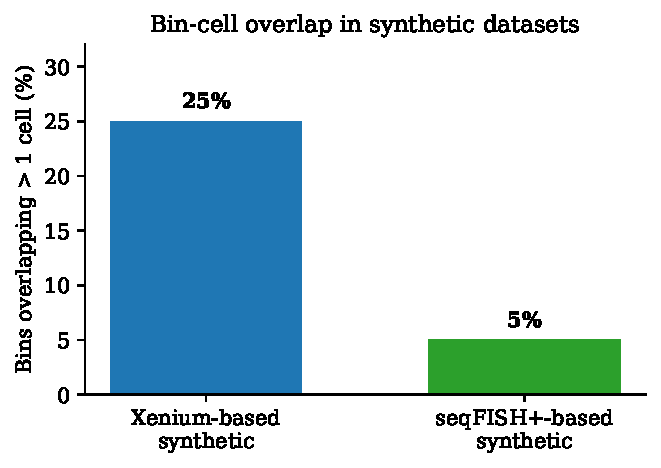
\includegraphics[width=0.55\textwidth]{figures/fig2_overlap.pdf}
\caption{Fraction of Visium HD bins that overlap more than one cell in the two synthetic datasets used for evaluation. On the Xenium-based synthetic dataset with whole-cell boundaries, about 25\% of bins overlap more than one cell, driving low recall for the Naive assignment strategy. On the seqFISH+-based synthetic dataset, only about 5\% of bins overlap more than one cell, so all four strategies perform comparably.}
\label{fig:overlap}
\end{figure}

When the evaluation is restricted to cell nuclei rather than whole cells, the gap between the Naive and the weighted methods narrows substantially. Fewer bins overlap more than one nucleus because nuclei are smaller and more separated than whole cells, limiting the benefit of the weighted methods over Naive. All four methods also achieve lower precision on nuclei than on whole cells, reflecting the fact that a larger fraction of bins near the nuclear boundary in fact contain transcripts originating in the cytoplasm.

The picture is quite different on the seqFISH+-based synthetic dataset, which targets NIH-3T3 cells that are relatively large and sparse. Here each cell intersects between roughly 200 and 700 bins, and only about 5\% of bins overlap more than one cell. Consequently, all four assignment strategies achieve precision close to 1 and recall close to 0.99. In this regime the Naive method is preferable in practice because it runs in shorter wall-clock time while matching the accuracy of the weighted variants. Taken together, these results establish that the choice between Naive and weight-based assignment should be driven by tissue density: dense, overlap-heavy tissues benefit from the weighted schemes, whereas sparse tissues can safely use the faster Naive method.

\subsection{Cell-Type Annotation Against Pathologist Labels}

Having characterised the four assignment strategies in isolation, we next asked how they interact with the three cell-type annotators when the pipeline is run end-to-end on real tissue with independent ground truth. We ran all twelve combinations of bin-to-cell strategy and annotator on a cohort of 20{,}991 pathologist-annotated cells drawn from human colorectal cancer and mouse small intestine samples, relabelling the more granular predictions of CellAssign, CellTypist and Sargent onto the three broad categories used by the pathologist---Epithelial, Stromal, and Immune---via a fixed mapping. Performance was measured as a three-class classifier using accuracy, precision, recall, and weighted F1, with gene markers sourced from a combination of expert input and PanglaoDB~\cite{franzen2019panglaodb} for Sargent and CellAssign.

Two consistent patterns emerged. First, the weight-based assignment methods consistently outperform the Naive method across all three annotators, yielding higher accuracy, precision, recall, and weighted F1. This shows that improvements in bin-to-cell assignment propagate to downstream cell-type annotation and are not merely reshuffled between annotator categories. Second, the choice of annotator matters as much as the choice of bin-to-cell strategy: Sargent is the best performer overall, followed by CellTypist, with CellAssign last. The best configuration pairs Sargent with the Weighted-by-Area assignment and yields accuracy 0.708 and weighted F1 0.758 on the 20{,}991-cell cohort (Figure~\ref{fig:bestperf}, Table~\ref{tab:bestperf}).

\begin{figure}[htbp]
\centering
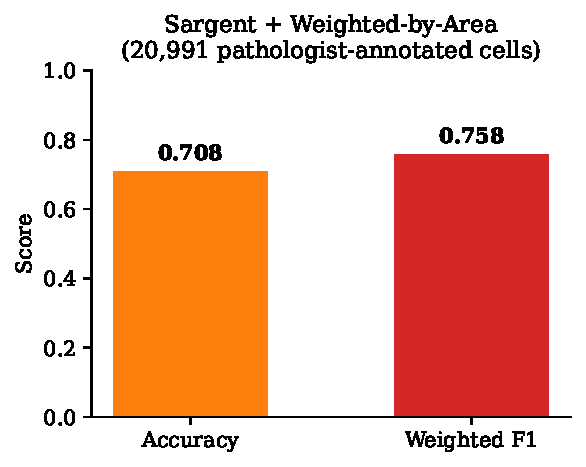
\includegraphics[width=0.55\textwidth]{figures/fig3_bestperf.pdf}
\caption{End-to-end cell-type classification performance of the best ENACT configuration (Sargent combined with Weighted-by-Area) on the cohort of 20{,}991 pathologist-annotated cells. Accuracy 0.708 and weighted F1 0.758.}
\label{fig:bestperf}
\end{figure}

\begin{table}[htbp]
\centering
\caption{Best end-to-end cell-type classification performance against pathologist labels.}
\label{tab:bestperf}
\begin{tabular}{lccc}
\toprule
Bin-to-cell + annotator & Number of cells & Accuracy & Weighted F1 \\
\midrule
Weighted-by-Area + Sargent & 20{,}991 & 0.708 & 0.758 \\
\bottomrule
\end{tabular}
\end{table}

The confusion-matrix structure across the twelve combinations is informative and largely explains the ranking of the annotators. CellAssign fails to identify immune cells, misclassifying them as epithelial; CellTypist also confuses a non-trivial fraction of immune cells with epithelial cells; Sargent, in contrast, differentiates immune and epithelial cells substantially better and concentrates its remaining errors on more ambiguous cell-type boundaries. All three annotators also emit a ``no label'' class for cells whose posterior or score does not exceed the model's threshold, which is a desirable property for exploratory studies in which the cell-type vocabulary is not fully known in advance. Some fraction of the residual error is likely attributable to heterogeneity in the pathologist's labels themselves---a region labelled ``epithelial'' can contain small immune or stromal aggregates---and to the choice of marker lists, which directly influences the output of Sargent and CellAssign.

\begin{table}[htbp]
\centering
\caption{Bin-cell overlap statistics on the two synthetic datasets.}
\label{tab:overlap}
\begin{tabular}{lc}
\toprule
Synthetic dataset & Bins overlapping $>1$ cell (\%) \\
\midrule
Xenium-based, whole-cell boundaries & 25 \\
seqFISH+-based, NIH-3T3 & $\sim 5$ \\
\bottomrule
\end{tabular}
\end{table}

\subsection{Cell-Type Enrichment in Anatomical Landmarks}

As a higher-level sanity check we asked whether the cells predicted by the best configuration (Weighted-by-Area plus Sargent) agree with pathologist-defined anatomical landmarks on the two real samples. For each landmark we identified the cell types ENACT assigned most frequently to cells inside that landmark, and compared the resulting lists to established biology of the respective tissues.

In the human colorectal cancer sample the dominant cell types in the ``muscular'' landmark are Smooth Muscle cells, B cells, and Fibroblasts; in the ``normal epithelial'' landmark they are Goblet, B, and Crypt cells; the ``tumoral epithelium'' landmark is dominated by Enterocytes, Goblet cells and B cells; and the ``stromal'' landmark by Fibroblasts, B cells and Endothelial cells. In the mouse small intestine sample the gene markers used by Sargent were tailored to mouse (supplementary Table~ST8). Here the ``muscular'' landmark is dominated by Smooth muscle cells and Paneth cells, the ``normal epithelium'' by Paneth, Goblet and B cells, and the ``lymphoid'' landmark is dominated by B cells. These correspondences are consistent with the known histology of both tissues: the mapping of B cells into apparently non-lymphoid landmarks is a known consequence of the pathologist's coarse region boundaries, which occasionally include small immune aggregates. Table~\ref{tab:landmarks} summarises the top predicted cell types per landmark.

\begin{table}[htbp]
\centering
\caption{Top predicted cell types per anatomical landmark for the best ENACT configuration (Weighted-by-Area + Sargent).}
\label{tab:landmarks}
\begin{tabular}{llp{6.5cm}}
\toprule
Tissue & Landmark & Top predicted cell types \\
\midrule
Human colorectal cancer & muscular & Smooth Muscle, B cells, Fibroblasts \\
Human colorectal cancer & normal epithelial & Goblet, B cells, Crypt \\
Human colorectal cancer & tumoral epithelium & Enterocytes, Goblet, B cells \\
Human colorectal cancer & stromal & Fibroblasts, B cells, Endothelial \\
Mouse small intestine & muscular & Smooth muscle, Paneth \\
Mouse small intestine & normal epithelium & Paneth, Goblet, B cells \\
Mouse small intestine & lymphoid & B cells \\
\bottomrule
\end{tabular}
\end{table}

\section{Discussion}

ENACT addresses a concrete bottleneck that has prevented Visium HD from reaching its promised single-cell resolution: the mismatch between the Visium HD grid and true cell boundaries. By coupling Stardist-based segmentation with four alternative bin-to-cell assignment strategies and three established cell-type annotators, the pipeline recovers per-cell transcript counts that are accurate enough to support downstream cell-type classification against independent pathology labels, and it packages the output into the Squidpy ecosystem without manual intervention. To our knowledge, ENACT is the first tissue-agnostic end-to-end pipeline that closes the loop from raw Visium HD bins to spatially-resolved cell types.

The principal empirical finding is that bin-to-cell assignment strategy should be chosen based on tissue density. On the Xenium-based synthetic where about 25\% of bins overlap more than one cell, the Weighted-by-Area method improves F1 over the Naive method by recovering ambiguous bins that the Naive method discards; on the seqFISH+-based synthetic where only about 5\% of bins overlap more than one cell, all four methods achieve near-identical precision and recall, and the faster Naive method is the pragmatic choice. This dependency on tissue density is biologically meaningful: dense epithelial and tumour samples are precisely the regions in which per-cell analysis is most valuable and where naive assignment fails hardest, so the weight-based methods close a gap that was most acute in the highest-value regime.

A second, complementary finding is that the choice of cell-type annotator has a first-order effect on end-to-end accuracy and interacts with bin-to-cell choice. Sargent, a score-based method, is the strongest annotator in our benchmark, consistent with the intuition that score-based methods cope better with sparse transcript counts than probabilistic methods such as CellAssign. CellAssign's failure to identify immune cells and CellTypist's confusion of immune with epithelial cells both stem partly from the comparatively low per-cell counts that Visium HD produces relative to standard scRNA-seq, for which these methods were originally calibrated. The observed ranking---Sargent ahead of CellTypist ahead of CellAssign---therefore reflects a property of the platform as much as it does a property of the algorithms, and argues for score-based annotation as the default in spatial assays.

The pipeline has several practical implications. Downstream analyses built on Squidpy, such as neighbourhood enrichment, Moran's I and co-occurrence tests, are immediately available once a sample has been processed through ENACT, so users inherit an entire ecosystem of spatial statistics without writing glue code. Equally important, ENACT produces paired imaging and gene-expression datasets on demand. Such paired datasets are the natural training material for next-generation vision-based cell classifiers that jointly exploit morphology and transcription, and doing so without manual per-cell annotation lifts the main practical barrier to assembling such datasets at scale. By making these outputs routine, ENACT contributes raw material to the broader single-cell and digital-pathology communities beyond the immediate Visium HD userbase.

Several limitations of the present study are important to acknowledge. The pathologist annotations used for end-to-end evaluation are labour-intensive and not error-free: regions labelled ``epithelial'' in the human colorectal cancer sample can contain small stromal or immune aggregates, which inflates apparent misclassification in the confusion matrices. The marker-based annotators (Sargent and CellAssign) depend on the quality of the marker list, and resources such as PanglaoDB and CellMarker encode known biases that propagate into the outputs. The synthetic datasets used for the bin-level evaluation project imaging-based transcripts onto a Visium HD grid; this captures the geometry of the problem but not every noise source of the actual Visium HD chemistry, so real-data precision and recall may differ from the synthetic numbers. Finally, cell segmentation quality is an upstream bottleneck that is hidden from our evaluation: any systematic error made by Stardist propagates directly into the assigned transcript counts, and improvements in segmentation are likely to translate one-to-one into improvements in downstream cell-type accuracy.

Several lines of future work follow naturally from these observations. First, the supplementary Section~1 methods for weight-based assignment could be extended with content-aware weights that use morphology rather than only geometric overlap, which would combine the strengths of imaging and sequencing more fully. Second, training vision-based classifiers on the paired datasets ENACT produces is a natural next step, and would let the morphological signal substitute for transcripts in samples where sequencing yield is low. Third, deploying ENACT across a wider tissue catalogue would allow systematic characterisation of the dependence of the best bin-to-cell strategy on tissue density, potentially enabling an automatic strategy selector that inspects the bin-overlap statistic (Figure~\ref{fig:overlap}) of a new sample and picks Weighted-by-Area or Naive accordingly. Taken together, these directions suggest that ENACT is both a usable tool and a foundation on which a richer generation of Visium HD analyses can be built: it turns a raw Visium HD bin-by-gene matrix into a ready-to-analyse AnnData object, it connects directly into the Scanpy and Squidpy ecosystems, and it produces the paired imaging-plus-transcriptomics datasets that will drive the next generation of vision-based cell classifiers. ENACT is released as an open-source Python package.

\bibliographystyle{unsrtnat}
\bibliography{references}

\end{document}
